\documentclass{beamer}
\mode<presentation>
\usepackage{amsmath}
\usepackage{amssymb}
%\usepackage{advdate}
\usepackage{adjustbox}
\usepackage{subcaption}
\usepackage{enumitem}
\usepackage{multicol}
\usepackage{gensymb}
\usepackage{mathtools}
\usepackage{listings}
\usepackage{url}
\def\UrlBreaks{\do\/\do-}
\usetheme{Boadilla}
\usecolortheme{lily}
\setbeamertemplate{footline}
{
  \leavevmode%
  \hbox{%
  \begin{beamercolorbox}[wd=\paperwidth,ht=2ex,dp=1ex,right]{author in head/foot}%
    \insertframenumber{} / \inserttotalframenumber\hspace*{2ex} 
  \end{beamercolorbox}}%
  \vskip0pt%
}
\setbeamertemplate{navigation symbols}{}

\providecommand{\nCr}[2]{\,^{#1}C_{#2}} % nCr
\providecommand{\nPr}[2]{\,^{#1}P_{#2}} % nPr
\providecommand{\mbf}{\mathbf}
\providecommand{\pr}[1]{\ensuremath{\Pr\left(#1\right)}}
\providecommand{\qfunc}[1]{\ensuremath{Q\left(#1\right)}}
\providecommand{\sbrak}[1]{\ensuremath{{}\left[#1\right]}}
\providecommand{\lsbrak}[1]{\ensuremath{{}\left[#1\right.}}
\providecommand{\rsbrak}[1]{\ensuremath{{}\left.#1\right]}}
\providecommand{\brak}[1]{\ensuremath{\left(#1\right)}}
\providecommand{\lbrak}[1]{\ensuremath{\left(#1\right.}}
\providecommand{\rbrak}[1]{\ensuremath{\left.#1\right)}}
\providecommand{\cbrak}[1]{\ensuremath{\left\{#1\right\}}}
\providecommand{\lcbrak}[1]{\ensuremath{\left\{#1\right.}}
\providecommand{\rcbrak}[1]{\ensuremath{\left.#1\right\}}}
\theoremstyle{remark}
\newtheorem{rem}{Remark}
\newcommand{\sgn}{\mathop{\mathrm{sgn}}}
\providecommand{\abs}[1]{\left\vert#1\right\vert}
\providecommand{\res}[1]{\Res\displaylimits_{#1}} 
\providecommand{\norm}[1]{\lVert#1\rVert}
\providecommand{\mtx}[1]{\mathbf{#1}}
\providecommand{\mean}[1]{E\left[ #1 \right]}
\providecommand{\fourier}{\overset{\mathcal{F}}{ \rightleftharpoons}}
%\providecommand{\hilbert}{\overset{\mathcal{H}}{ \rightleftharpoons}}
\providecommand{\system}{\overset{\mathcal{H}}{ \longleftrightarrow}}
	%\newcommand{\solution}[2]{\textbf{Solution:}{#1}}
%\newcommand{\solution}{\noindent \textbf{Solution: }}
\providecommand{\dec}[2]{\ensuremath{\overset{#1}{\underset{#2}{\gtrless}}}}
\newcommand{\myvec}[1]{\ensuremath{\begin{pmatrix}#1\end{pmatrix}}}
\let\vec\mathbf

\lstset{
%language=C,
frame=single, 
breaklines=true,
columns=fullflexible
}

\numberwithin{equation}{section}

\title{12.6.5.11 Presentation}
\author{G. Abhimanyu Koushik \\ EE24BTECH11024}

\date{\today} 
\begin{document}

\begin{frame}
\titlepage
\end{frame}

\section*{Outline}
\begin{frame}
\tableofcontents
\end{frame}
\section{Problem}
\begin{frame}
\frametitle{Problem Statement}
%
It is given that at $x = 1$, the function $x^4 - 62x^2 + ax + 9$ attains its maximum value, on the interval [0, 2]. Find the value of a.
%
\end{frame}

%\subsection{Literature}
\section{Solution}
\subsection{Theoritical Solution}
\begin{frame}
\frametitle{Theoritical Solution}
%\framesubtitle{Literature}
Given function
\begin{align}
	f\brak{x} = x^4 - 62x^2 + ax + 9
\end{align}
If a function has a local maxima at $x=x_0$ then $f^\prime\brak{x_0} = 0$ and $f^{\prime\prime}\brak{x_0} \le 0$
\begin{align}
	f^\prime\brak{x} = 4x^3 - 124x + a \\
	f^{\prime\prime}\brak{x} = 12x^2 - 124\\
	f^\prime\brak{1} = 4-124+a\\
	f^{\prime\prime}\brak{1} = 12 - 124
\end{align}
$f^{\prime\prime}\brak{1}$ is anyway negative so $f^\prime\brak{1}$ should be $0$
\begin{align}
	a-120 =0\\
	a = 120
\end{align}
When $a = 120$, it satisfies all the conditions.\\
\end{frame}
\subsection{Computational Solution}
\begin{frame}
\frametitle{Computational Solution}
Given function
\begin{align}
	f\brak{x} = x^4 - 62x^2 + ax + 9
\end{align}
At any critical point $x=x_0$, $\brak{f^\prime\brak{x_0}}^2$ is minimum. We need to minimize
\begin{align}
L\brak{a} = \brak{f^\prime\brak{1}}^2\\
L\brak{a} = \brak{a-120}^2
\end{align}
We use the method of gradient descent to find the minimum of the above function, since the objective function is convex.
\begin{align}
    a_{n+1} &= a_n - \mu L^{\prime}\brak{a_n}\\
    L^{\prime}\brak{a_n} &= 2\brak{a_n-120}\\
    \xrightarrow{} a_{n+1} &= a_n - 2\mu\brak{a_n-120}
\end{align}
\end{frame}
\begin{frame}
Applying unilateral Z-transform,
\begin{align}
    zX\brak{z} - zx_0 &= \brak{1-2\mu}X\brak{z}+\frac{240\mu}{1-z^{-1}}
\end{align}
The Unilateral Z-transform of a constant function $f\brak{x} = c$ is $\frac{c}{1-z^{-1}}$ with Radius of convergence being $\abs{z}>1$
\begin{align}
    \brak{z - \brak{1-2\mu}}X\brak{z} = zx_0+\frac{240\mu}{1-z^{-1}}\\
    X\brak{z} = \frac{zx_0}{z - \brak{1-2\mu}}+\frac{240\mu}{\brak{1-z^{-1}}\brak{z - \brak{1-2\mu}}}\\
    X\brak{z} = \frac{x_0}{1 - \brak{1-2\mu}z^{-1}}+\frac{240\mu}{z-2\brak{1-\mu}+\brak{1-2\mu}z^{-1}}\\
    X\brak{z} = \frac{x_0}{1 - \brak{1-2\mu}z^{-1}}+\frac{240\mu z^{-1}}{1-2\brak{1-\mu}z^{-1}+\brak{1-2\mu}z^{-2}}\\
    = \sum_{0}^{\infty} \brak{1-2\mu}^n z^{-n}+\sum_{1}^{\infty}\frac{1-\brak{1-2\mu}^n}{2\mu}z^{-n}\\
    = \sum_{0}^{\infty} \brak{1-2\mu}^n z^{-n}+\sum_{1}^{\infty}\frac{1}{2\mu}z^{-n}-\sum_{1}^{\infty}\frac{\brak{1-2\mu}^n}{2\mu}z^{-n}\\
\end{align}
\end{frame}
\begin{frame}
From the last equation, ROC is 
\begin{align}
    \abs{z} &> \abs{1-2\mu}\\
    \abs{z} &> 1 \\
    \xrightarrow{} 0 < |1-2\mu| < 1\\
    \xrightarrow{} \mu \in \brak{0, \frac{1}{2}}
\end{align}
Now, if $\mu$ satisfies the previous condition,
\begin{align}
    \lim_{n \to \infty} \brak{a_{n+1} - a_n} = 0\\
    \xrightarrow{} \lim_{n \to \infty} \brak{- 2\mu\brak{a_n-120}} = 0\\
    \xrightarrow{} {-2\mu}\lim_{n \to \infty} \brak{a_n-120} = 0\\
    \xrightarrow{} \lim_{n \to \infty} \brak{a_n} = 120\\
    \xrightarrow{} \lim_{n \to \infty} a_n = 120
\end{align}
\end{frame}
\begin{frame}
Taking initial guess = 50\\ step size = 0.1\\ tolerance(minimum value of gradient) = 1e-5\\ We get \\
$a_{min} = 119.99999528200934$\\
\end{frame}
\subsection{Quadratic Programming}
\begin{frame}
\frametitle{Quadratic Programming}
The question minimum value of $L\brak{a} = \brak{a-120}^2$ can be viewed as a Quadratic Programming problem as:\\
\begin{align}
    \min_{\vec{x}} \abs{e_2^{\top}\vec{x}}\\
    \text{s.t. } \\ \vec{x}^{\top}V\vec{x} + 2\vec{u}^{\top}\vec{x} + f = 0\\
    V = \myvec{1 & 0 \\ 0 & 0}\\
    \vec{u} = \myvec{-120 \\ -0.5}\\
    f = 14400
\end{align}
\end{frame}
\begin{frame}
The constraint here is non-convex since the constraint defines a set which is not convex, since points on the
line joining any 2 points on the curve don't belong to the set. However, if we make the constraint
\begin{align}
    \vec{x}^{\top}V\vec{x} + 2\vec{u}^{\top}\vec{x} + f\le 0
\end{align}
the constraint becomes convex. Using cvxpy to solve this convex optimization problem, we get \\
\begin{align}
    Optimal x: [[ 1.19999997e+02]\\
 [-3.74242669e-05]]
\end{align}
\end{frame}
\section{Plots}
\begin{frame}
\frametitle{Plot}
\begin{figure}[h!]
   \centering
   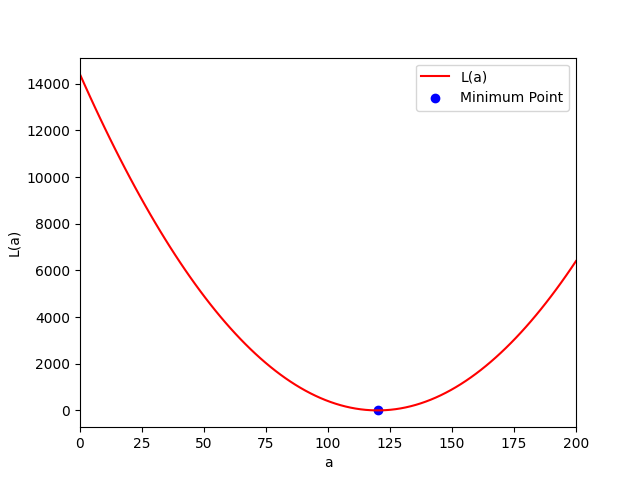
\includegraphics[width=0.8\columnwidth]{figs/fig1.png}
   \caption{Graph of $L\brak{a} = \brak{a - 120}^2$ and the value of $a$ which satisfies the given conditions}
   \label{stemplot}
\end{figure}
\end{frame}
\begin{frame}
\begin{figure}[h!]
   \centering
   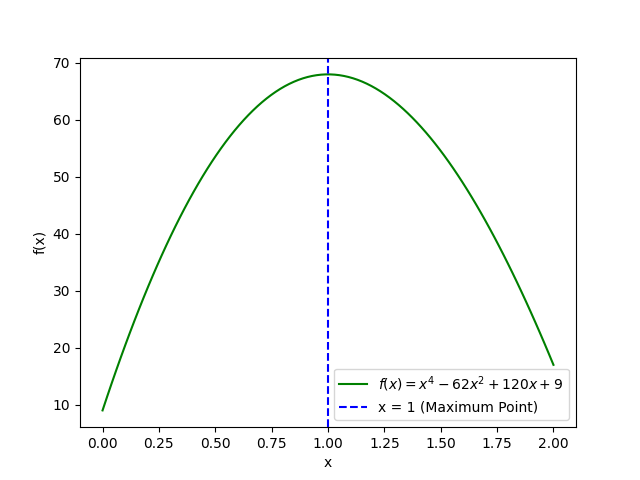
\includegraphics[width=0.8\columnwidth]{figs/fig2.png}
   \caption{Graph of $f\brak{x}$ when $a = 120$}
   \label{stemplot}
\end{figure}
\end{frame}
\end{document}

